\documentclass[conference]{IEEEtran}
\usepackage[T1]{fontenc}
\usepackage[utf8]{inputenc}
\usepackage{times}
\usepackage{microtype}
\usepackage{graphicx}
\usepackage{booktabs}
\usepackage{amsmath}
\usepackage{cite}
\usepackage[hidelinks]{hyperref}
\usepackage{tikz}
\usetikzlibrary{arrows.meta,positioning,fit,calc,matrix}

\definecolor{ink}{HTML}{1F2328}
\definecolor{muted}{HTML}{5E6168}
\definecolor{rule}{HTML}{D9D7D0}
\definecolor{ordblue}{HTML}{2A78D6}
\definecolor{deporange}{HTML}{EB6834}
\definecolor{lenaqua}{HTML}{1BAF7A}
\definecolor{rowlab}{HTML}{E3A600}
\definecolor{colhead}{HTML}{C9CCD1}
\tikzset{
  stage/.style={draw=muted,rounded corners=2pt,fill=white,align=center,font=\scriptsize,minimum height=7mm,inner xsep=1pt,text width=12.5mm},
  hot/.style={stage,draw=deporange,line width=.9pt},
  flow/.style={-{Stealth[length=1.6mm]},muted},
}

\begin{document}
\title{Dependency-Preserving Evidence Packing\\for Numerical Question Answering over Financial Reports}
\author{\IEEEauthorblockN{Pushpendra Singh \qquad Badri Bishal Das}
\IEEEauthorblockA{Indian Institute of Technology Guwahati\\Big Data course project}}
\maketitle

\begin{abstract}
A language model answering questions about a financial report sees only the evidence
that fits its context window. The answers sit in tables, and a table cell is
meaningless without its row and column labels. Dropping the labels makes numbers
ambiguous; repeating them with every number costs 2.2 to 8.3 times more tokens per
cell and pushes needed numbers out of the window. We represent each report as a
dependency graph in which every number links to the labels it needs, and pack evidence
so that each label is written once and shared. A PySpark pipeline builds and verifies
the graph for six datasets: 1.36 million facts and 1.88 million label links. Over all
9,268 development questions, the method keeps the gold evidence more often than
label-repeating packing on all six datasets, by 0.3 to 4.0 points at the chosen
budgets. The gain closes as budgets grow and reverses at a 200-token budget. With
Gemini 3.5 Flash-Lite, answers are at least as good on all six datasets and better on
TAT-QA by 11.3 points.
\end{abstract}

\section{Introduction}
Analysts query annual reports for specific numbers: a margin, a growth rate, a ratio
of two line items. Answering such questions is table--text hybrid question answering.
A large language model (LLM) can do it, but only from the text in its prompt, and a
report is far longer than the evidence budget a system gives the model. The system
must retrieve a few facts and \emph{pack} them into that budget.

Tables make this hard. Fig.~\ref{fig:example} shows a real FinQA table. The question
asks for American Express's average payment volume per transaction. A retriever ranks
637 and 647 highest; only their column headers say that the first is payments volume
and the second total volume. Packed without labels, the two are interchangeable.
Packed with all their labels, as in serializations such as ``the revenue of 2019 is
100''~\cite{arun2023}, each cell costs several times more and fewer cells fit. We need
packing that keeps every number's labels and still fits the budget.

\begin{figure}[t]
\centering
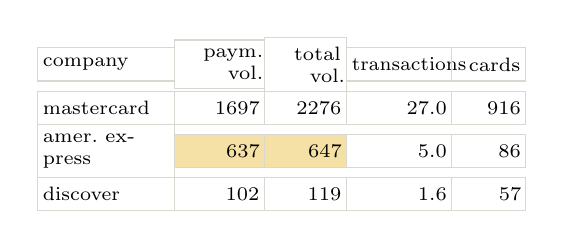
\begin{tikzpicture}[font=\scriptsize]
\matrix (t) [matrix of nodes, nodes={draw=rule,minimum height=4.2mm,inner xsep=2pt,anchor=center},
  column sep=-\pgflinewidth, row sep=-\pgflinewidth,
  column 1/.style={nodes={text width=16mm}}, column 2/.style={nodes={text width=10mm,align=right}},
  column 3/.style={nodes={text width=9mm,align=right}}, column 4/.style={nodes={text width=12mm,align=right}},
  column 5/.style={nodes={text width=8mm,align=right}}]{
  company & paym.\ vol. & total vol. & transactions & cards\\
  mastercard & 1697 & 2276 & 27.0 & 916\\
  amer.\ express & |[fill=rowlab!35]| 637 & |[fill=rowlab!35]| 647 & 5.0 & 86\\
  discover & 102 & 119 & 1.6 & 57\\
};
\end{tikzpicture}\\[2pt]
{\scriptsize ``What is the average payment volume per transaction for American Express?''
$637 \div 5.0 = 127.4$.}
\caption{Running example from the FinQA development set (V/2008/page\_17, rows
abridged). The two top-ranked cells differ only by their column header.}
\label{fig:example}
\end{figure}

\textbf{Contributions.}
\begin{itemize}
\item Dependency-preserving packing: each number is admitted with the labels it points
to, and a label already packed costs nothing. We give its exact token trade-off: a
fixed cost for structure, then cells 2.2 to 8.3 times cheaper.
\item A PySpark data layer that normalises six datasets into one verified store of
facts and label links.
\item A coverage audit over all 9,268 development questions, five budgets and three
packing methods, with no model in the loop.
\item A paired answer experiment with Gemini 3.5 Flash-Lite, in which the model copies
numbers and code checks and computes them.
\end{itemize}

\section{Problem statement and objectives}
The assigned problem is numerical reasoning over financial reports on FinQA, TAT-QA,
ConvFinQA and HybridQA. Our question: \emph{with the same model and the same evidence
budget, does keeping each number's headers, units, hierarchy and links improve answers
over packing that repeats labels inline?} The hypothesis predicts two limits. Labels
consume budget, so the method can lose when almost nothing fits; when the whole document
fits, there is nothing to choose. Objectives: (O1) one pipeline over the four assigned
datasets plus TAT-HQA and MultiHiertt, scored by the official evaluators; (O2)
dependency-preserving packing against label-repeating and length-matched baselines at
a fixed budget; (O3) a verified PySpark preparation of all six datasets; (O4) a paired
answer test; (O5) answers grounded in the evidence.

\section{Datasets}
We use the development splits of six datasets (Table~\ref{tab:data}), each from its
official repository at a pinned commit, with the supplied document context and the
official scorers. FinQA and ConvFinQA share documents, as do TAT-QA and TAT-HQA, so we
never pool results. HybridQA is Wikipedia rather than finance and tests whether the
method transfers. Passing gold answers from 200 development questions through each
scorer gives 100\% on five datasets and 90.5\% on MultiHiertt, whose span path drops
minus signs.
\begin{table}[t]
\centering\footnotesize\setlength{\tabcolsep}{4pt}
\caption{Development data. D and O: median document size in tokens with each label
written once and with labels repeated in every cell.}
\label{tab:data}
\begin{tabular}{lrlrrr}
\toprule
Dataset & Questions & Challenge & D & O & Budget\\\midrule
FinQA & 883 & programs & 1,041 & 1,112 & 800\\
ConvFinQA & 1,490 turns & history & 979 & 1,062 & 800\\
TAT-QA & 1,668 & spans, scale & 396 & 592 & 400\\
TAT-HQA & 824 & hypotheticals & 396 & 592 & 400\\
HybridQA & 3,466 & passage links & 8,928 & 11,142 & 1,500\\
MultiHiertt & 1,044 & hierarchy & 3,693 & 6,435 & 1,500\\
\bottomrule
\end{tabular}\\[2pt]
{\scriptsize Sources (GitHub): czyssrs/FinQA, czyssrs/ConvFinQA, NExTplusplus/TAT-QA,
NExTplusplus/TAT-HQA, wenhuchen/HybridQA, psunlpgroup/MultiHiertt.}
\end{table}

\section{Proposed methodology}
Fig.~\ref{fig:pipeline} shows the pipeline. Only the packing step differs between the
three methods we compare.

\begin{figure}[t]
\centering
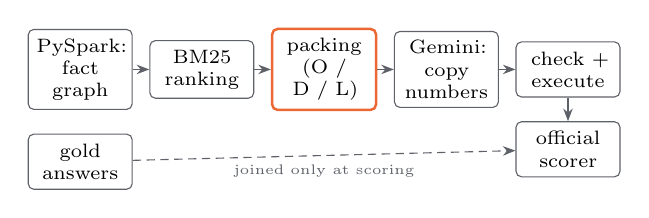
\begin{tikzpicture}[node distance=2.1mm]
\node[stage] (o1) {PySpark:\\fact graph};
\node[stage,right=of o1] (o2) {BM25\\ranking};
\node[hot,right=of o2] (o3) {packing\\(O / D / L)};
\node[stage,right=of o3] (o4) {Gemini:\\copy numbers};
\node[stage,right=of o4] (o5) {check +\\execute};
\foreach \a/\b in {o1/o2,o2/o3,o3/o4,o4/o5}\draw[flow] (\a)--(\b);
\node[stage,below=3mm of o1] (g) {gold answers};
\node[stage,below=3mm of o5] (s) {official\\scorer};
\draw[flow] (o5)--(s);
\draw[flow,densely dashed] (g)--(s) node[midway,below,font=\tiny,muted] {joined only at scoring};
\end{tikzpicture}
\caption{Pipeline. The highlighted step is the only one that varies.}
\label{fig:pipeline}
\end{figure}

\subsection{Evidence as a dependency graph}
Readers turn each document into \emph{facts}: raw text, provenance, and the IDs of the
facts needed to read it (Fig.~\ref{fig:graph}). A table cell depends on its column
header, row label, corner header and section row. TAT-QA cells also depend on unit
paragraphs (``in thousands''); a HybridQA passage depends on the cell that links to
it; MultiHiertt cells depend on multi-row HTML headers and section headings. Headers are
inferred from layout and flagged uncertain. Gold answers never enter prompts: none of
443 inspected prompts contains a gold label field.

\begin{figure}[t]
\centering
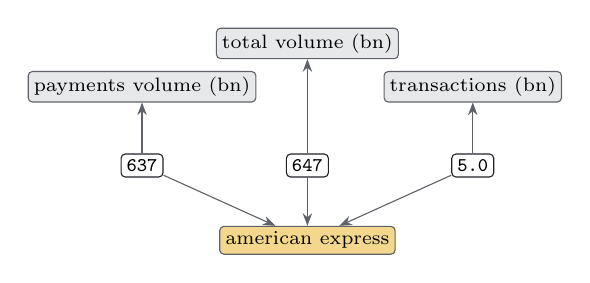
\begin{tikzpicture}[font=\scriptsize,
  fact/.style={draw=ink,rounded corners=1.5pt,fill=white,inner sep=2pt,font=\scriptsize\ttfamily},
  lab/.style={draw=muted,rounded corners=1.5pt,fill=colhead!45,inner sep=2pt}]
\node[fact] (a) at (0,0) {637};
\node[fact] (b) at (2.1,0) {647};
\node[fact] (c) at (4.2,0) {5.0};
\node[lab] (ha) at (0,1.0) {payments volume (bn)};
\node[lab] (hb) at (2.1,1.55) {total volume (bn)};
\node[lab] (hc) at (4.2,1.0) {transactions (bn)};
\node[lab,fill=rowlab!45] (row) at (2.1,-0.95) {american express};
\foreach \x/\h in {a/ha,b/hb,c/hc}\draw[flow] (\x)--(\h);
\foreach \x in {a,b,c}\draw[flow] (\x)--(row);
\end{tikzpicture}
\caption{Dependency graph for three cells of the running example. The row label is a
single shared node.}
\label{fig:graph}
\end{figure}

\subsection{Packing under the budget}
BM25 ranks cells and paragraphs by the question and earlier questions. Candidates are
admitted in rank order as whole bundles; strings are never cut, and a bundle that does
not fit is skipped so smaller ones can still enter. Three methods spend the same budget:
\begin{itemize}
\item \textbf{Ordinary (O)}: each fact carries its structural labels inline. Labels are
kept, so the baseline is fair.
\item \textbf{Dependency (D)}: each fact enters with the recursive closure of its
headers, units, hierarchy and link anchors; packed labels are free.
\item \textbf{Length-matched (L)}: ordinary facts plus their document neighbours, up to
D's token count. It tests whether more text alone helps.
\end{itemize}
Tokens are counted locally on the evidence text as UTF-8 bytes divided by four.

Fig.~\ref{fig:strips} shows the trade-off. D's first cell costs 18 tokens against O's
15 because its headers come with it; four cells cost 50 against 57. L spends its tokens
on a neighbouring Mastercard cell and loses 5.0. Across all development tables, a
labelled cell costs 15.1 tokens in FinQA against 3.6 bare (4.2$\times$), 15.6 against
7.0 in HybridQA, and 24.7 against 3.0 in MultiHiertt (8.3$\times$). The median TAT-QA
document needs 396 tokens with labels once and 592 with labels repeated; its budget is
400 (Table~\ref{tab:data}).

\begin{figure}[t]
\centering
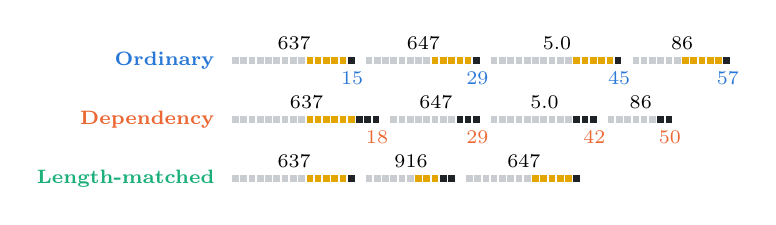
\begin{tikzpicture}[font=\scriptsize]
\node[anchor=east,text=ordblue,font=\scriptsize\bfseries] at (-0.1,0.04) {Ordinary};
\fill[colhead] (0.000,0.000) rectangle ++(0.085,0.085);
\fill[colhead] (0.105,0.000) rectangle ++(0.085,0.085);
\fill[colhead] (0.210,0.000) rectangle ++(0.085,0.085);
\fill[colhead] (0.315,0.000) rectangle ++(0.085,0.085);
\fill[colhead] (0.420,0.000) rectangle ++(0.085,0.085);
\fill[colhead] (0.525,0.000) rectangle ++(0.085,0.085);
\fill[colhead] (0.630,0.000) rectangle ++(0.085,0.085);
\fill[colhead] (0.735,0.000) rectangle ++(0.085,0.085);
\fill[colhead] (0.840,0.000) rectangle ++(0.085,0.085);
\fill[rowlab] (0.945,0.000) rectangle ++(0.085,0.085);
\fill[rowlab] (1.050,0.000) rectangle ++(0.085,0.085);
\fill[rowlab] (1.155,0.000) rectangle ++(0.085,0.085);
\fill[rowlab] (1.260,0.000) rectangle ++(0.085,0.085);
\fill[rowlab] (1.365,0.000) rectangle ++(0.085,0.085);
\fill[ink] (1.470,0.000) rectangle ++(0.085,0.085);
\node[above] at (0.787,0.06) {637};
\node[below,text=ordblue] at (1.525,0.02) {15};
\fill[colhead] (1.695,0.000) rectangle ++(0.085,0.085);
\fill[colhead] (1.800,0.000) rectangle ++(0.085,0.085);
\fill[colhead] (1.905,0.000) rectangle ++(0.085,0.085);
\fill[colhead] (2.010,0.000) rectangle ++(0.085,0.085);
\fill[colhead] (2.115,0.000) rectangle ++(0.085,0.085);
\fill[colhead] (2.220,0.000) rectangle ++(0.085,0.085);
\fill[colhead] (2.325,0.000) rectangle ++(0.085,0.085);
\fill[colhead] (2.430,0.000) rectangle ++(0.085,0.085);
\fill[rowlab] (2.535,0.000) rectangle ++(0.085,0.085);
\fill[rowlab] (2.640,0.000) rectangle ++(0.085,0.085);
\fill[rowlab] (2.745,0.000) rectangle ++(0.085,0.085);
\fill[rowlab] (2.850,0.000) rectangle ++(0.085,0.085);
\fill[rowlab] (2.955,0.000) rectangle ++(0.085,0.085);
\fill[ink] (3.060,0.000) rectangle ++(0.085,0.085);
\node[above] at (2.430,0.06) {647};
\node[below,text=ordblue] at (3.115,0.02) {29};
\fill[colhead] (3.285,0.000) rectangle ++(0.085,0.085);
\fill[colhead] (3.390,0.000) rectangle ++(0.085,0.085);
\fill[colhead] (3.495,0.000) rectangle ++(0.085,0.085);
\fill[colhead] (3.600,0.000) rectangle ++(0.085,0.085);
\fill[colhead] (3.705,0.000) rectangle ++(0.085,0.085);
\fill[colhead] (3.810,0.000) rectangle ++(0.085,0.085);
\fill[colhead] (3.915,0.000) rectangle ++(0.085,0.085);
\fill[colhead] (4.020,0.000) rectangle ++(0.085,0.085);
\fill[colhead] (4.125,0.000) rectangle ++(0.085,0.085);
\fill[colhead] (4.230,0.000) rectangle ++(0.085,0.085);
\fill[rowlab] (4.335,0.000) rectangle ++(0.085,0.085);
\fill[rowlab] (4.440,0.000) rectangle ++(0.085,0.085);
\fill[rowlab] (4.545,0.000) rectangle ++(0.085,0.085);
\fill[rowlab] (4.650,0.000) rectangle ++(0.085,0.085);
\fill[rowlab] (4.755,0.000) rectangle ++(0.085,0.085);
\fill[ink] (4.860,0.000) rectangle ++(0.085,0.085);
\node[above] at (4.125,0.06) {5.0};
\node[below,text=ordblue] at (4.915,0.02) {45};
\fill[colhead] (5.085,0.000) rectangle ++(0.085,0.085);
\fill[colhead] (5.190,0.000) rectangle ++(0.085,0.085);
\fill[colhead] (5.295,0.000) rectangle ++(0.085,0.085);
\fill[colhead] (5.400,0.000) rectangle ++(0.085,0.085);
\fill[colhead] (5.505,0.000) rectangle ++(0.085,0.085);
\fill[colhead] (5.610,0.000) rectangle ++(0.085,0.085);
\fill[rowlab] (5.715,0.000) rectangle ++(0.085,0.085);
\fill[rowlab] (5.820,0.000) rectangle ++(0.085,0.085);
\fill[rowlab] (5.925,0.000) rectangle ++(0.085,0.085);
\fill[rowlab] (6.030,0.000) rectangle ++(0.085,0.085);
\fill[rowlab] (6.135,0.000) rectangle ++(0.085,0.085);
\fill[ink] (6.240,0.000) rectangle ++(0.085,0.085);
\node[above] at (5.715,0.06) {86};
\node[below,text=ordblue] at (6.295,0.02) {57};
\node[anchor=east,text=deporange,font=\scriptsize\bfseries] at (-0.1,-0.71) {Dependency};
\fill[colhead] (0.000,-0.750) rectangle ++(0.085,0.085);
\fill[colhead] (0.105,-0.750) rectangle ++(0.085,0.085);
\fill[colhead] (0.210,-0.750) rectangle ++(0.085,0.085);
\fill[colhead] (0.315,-0.750) rectangle ++(0.085,0.085);
\fill[colhead] (0.420,-0.750) rectangle ++(0.085,0.085);
\fill[colhead] (0.525,-0.750) rectangle ++(0.085,0.085);
\fill[colhead] (0.630,-0.750) rectangle ++(0.085,0.085);
\fill[colhead] (0.735,-0.750) rectangle ++(0.085,0.085);
\fill[colhead] (0.840,-0.750) rectangle ++(0.085,0.085);
\fill[rowlab] (0.945,-0.750) rectangle ++(0.085,0.085);
\fill[rowlab] (1.050,-0.750) rectangle ++(0.085,0.085);
\fill[rowlab] (1.155,-0.750) rectangle ++(0.085,0.085);
\fill[rowlab] (1.260,-0.750) rectangle ++(0.085,0.085);
\fill[rowlab] (1.365,-0.750) rectangle ++(0.085,0.085);
\fill[rowlab] (1.470,-0.750) rectangle ++(0.085,0.085);
\fill[ink] (1.575,-0.750) rectangle ++(0.085,0.085);
\fill[ink] (1.680,-0.750) rectangle ++(0.085,0.085);
\fill[ink] (1.785,-0.750) rectangle ++(0.085,0.085);
\node[above] at (0.945,-0.69) {637};
\node[below,text=deporange] at (1.840,-0.73) {18};
\fill[colhead] (2.010,-0.750) rectangle ++(0.085,0.085);
\fill[colhead] (2.115,-0.750) rectangle ++(0.085,0.085);
\fill[colhead] (2.220,-0.750) rectangle ++(0.085,0.085);
\fill[colhead] (2.325,-0.750) rectangle ++(0.085,0.085);
\fill[colhead] (2.430,-0.750) rectangle ++(0.085,0.085);
\fill[colhead] (2.535,-0.750) rectangle ++(0.085,0.085);
\fill[colhead] (2.640,-0.750) rectangle ++(0.085,0.085);
\fill[colhead] (2.745,-0.750) rectangle ++(0.085,0.085);
\fill[ink] (2.850,-0.750) rectangle ++(0.085,0.085);
\fill[ink] (2.955,-0.750) rectangle ++(0.085,0.085);
\fill[ink] (3.060,-0.750) rectangle ++(0.085,0.085);
\node[above] at (2.587,-0.69) {647};
\node[below,text=deporange] at (3.115,-0.73) {29};
\fill[colhead] (3.285,-0.750) rectangle ++(0.085,0.085);
\fill[colhead] (3.390,-0.750) rectangle ++(0.085,0.085);
\fill[colhead] (3.495,-0.750) rectangle ++(0.085,0.085);
\fill[colhead] (3.600,-0.750) rectangle ++(0.085,0.085);
\fill[colhead] (3.705,-0.750) rectangle ++(0.085,0.085);
\fill[colhead] (3.810,-0.750) rectangle ++(0.085,0.085);
\fill[colhead] (3.915,-0.750) rectangle ++(0.085,0.085);
\fill[colhead] (4.020,-0.750) rectangle ++(0.085,0.085);
\fill[colhead] (4.125,-0.750) rectangle ++(0.085,0.085);
\fill[colhead] (4.230,-0.750) rectangle ++(0.085,0.085);
\fill[ink] (4.335,-0.750) rectangle ++(0.085,0.085);
\fill[ink] (4.440,-0.750) rectangle ++(0.085,0.085);
\fill[ink] (4.545,-0.750) rectangle ++(0.085,0.085);
\node[above] at (3.968,-0.69) {5.0};
\node[below,text=deporange] at (4.600,-0.73) {42};
\fill[colhead] (4.770,-0.750) rectangle ++(0.085,0.085);
\fill[colhead] (4.875,-0.750) rectangle ++(0.085,0.085);
\fill[colhead] (4.980,-0.750) rectangle ++(0.085,0.085);
\fill[colhead] (5.085,-0.750) rectangle ++(0.085,0.085);
\fill[colhead] (5.190,-0.750) rectangle ++(0.085,0.085);
\fill[colhead] (5.295,-0.750) rectangle ++(0.085,0.085);
\fill[ink] (5.400,-0.750) rectangle ++(0.085,0.085);
\fill[ink] (5.505,-0.750) rectangle ++(0.085,0.085);
\node[above] at (5.190,-0.69) {86};
\node[below,text=deporange] at (5.560,-0.73) {50};
\node[anchor=east,text=lenaqua,font=\scriptsize\bfseries] at (-0.1,-1.46) {Length-matched};
\fill[colhead] (0.000,-1.500) rectangle ++(0.085,0.085);
\fill[colhead] (0.105,-1.500) rectangle ++(0.085,0.085);
\fill[colhead] (0.210,-1.500) rectangle ++(0.085,0.085);
\fill[colhead] (0.315,-1.500) rectangle ++(0.085,0.085);
\fill[colhead] (0.420,-1.500) rectangle ++(0.085,0.085);
\fill[colhead] (0.525,-1.500) rectangle ++(0.085,0.085);
\fill[colhead] (0.630,-1.500) rectangle ++(0.085,0.085);
\fill[colhead] (0.735,-1.500) rectangle ++(0.085,0.085);
\fill[colhead] (0.840,-1.500) rectangle ++(0.085,0.085);
\fill[rowlab] (0.945,-1.500) rectangle ++(0.085,0.085);
\fill[rowlab] (1.050,-1.500) rectangle ++(0.085,0.085);
\fill[rowlab] (1.155,-1.500) rectangle ++(0.085,0.085);
\fill[rowlab] (1.260,-1.500) rectangle ++(0.085,0.085);
\fill[rowlab] (1.365,-1.500) rectangle ++(0.085,0.085);
\fill[ink] (1.470,-1.500) rectangle ++(0.085,0.085);
\node[above] at (0.787,-1.44) {637};
\fill[colhead] (1.695,-1.500) rectangle ++(0.085,0.085);
\fill[colhead] (1.800,-1.500) rectangle ++(0.085,0.085);
\fill[colhead] (1.905,-1.500) rectangle ++(0.085,0.085);
\fill[colhead] (2.010,-1.500) rectangle ++(0.085,0.085);
\fill[colhead] (2.115,-1.500) rectangle ++(0.085,0.085);
\fill[colhead] (2.220,-1.500) rectangle ++(0.085,0.085);
\fill[rowlab] (2.325,-1.500) rectangle ++(0.085,0.085);
\fill[rowlab] (2.430,-1.500) rectangle ++(0.085,0.085);
\fill[rowlab] (2.535,-1.500) rectangle ++(0.085,0.085);
\fill[ink] (2.640,-1.500) rectangle ++(0.085,0.085);
\fill[ink] (2.745,-1.500) rectangle ++(0.085,0.085);
\node[above] at (2.272,-1.44) {916};
\fill[colhead] (2.970,-1.500) rectangle ++(0.085,0.085);
\fill[colhead] (3.075,-1.500) rectangle ++(0.085,0.085);
\fill[colhead] (3.180,-1.500) rectangle ++(0.085,0.085);
\fill[colhead] (3.285,-1.500) rectangle ++(0.085,0.085);
\fill[colhead] (3.390,-1.500) rectangle ++(0.085,0.085);
\fill[colhead] (3.495,-1.500) rectangle ++(0.085,0.085);
\fill[colhead] (3.600,-1.500) rectangle ++(0.085,0.085);
\fill[colhead] (3.705,-1.500) rectangle ++(0.085,0.085);
\fill[rowlab] (3.810,-1.500) rectangle ++(0.085,0.085);
\fill[rowlab] (3.915,-1.500) rectangle ++(0.085,0.085);
\fill[rowlab] (4.020,-1.500) rectangle ++(0.085,0.085);
\fill[rowlab] (4.125,-1.500) rectangle ++(0.085,0.085);
\fill[rowlab] (4.230,-1.500) rectangle ++(0.085,0.085);
\fill[ink] (4.335,-1.500) rectangle ++(0.085,0.085);
\node[above] at (3.705,-1.44) {647};
\end{tikzpicture}
\\[3pt]
{\scriptsize
\tikz\fill[colhead] (0,0) rectangle (.15,.15); column header\quad
\tikz\fill[rowlab] (0,0) rectangle (.15,.15); row label\quad
\tikz\fill[ink] (0,0) rectangle (.15,.15); value\quad one square = one token}
\caption{Packing the American Express row. Numbers below each group are cumulative
tokens.}
\label{fig:strips}
\end{figure}

\subsection{Grounded answers}
The model returns a JSON plan of official operations whose arguments are numbers copied
from the evidence, e.g.\ \texttt{divide("637","5.0")}. Code locates each number in the
packed evidence or the question, rejects the plan if one is missing, and computes the
result in a bounded decimal interpreter. Grounding blocks invented numbers but not
wrong real ones: \texttt{divide("647","5.0")} passes and returns 129.4. Labels are what
prevent that choice.

\section{Big Data implementation with PySpark}
The six datasets come as JSON (FinQA, TAT-QA, TAT-HQA), a zip archive (ConvFinQA),
HTML tables (MultiHiertt) and a linked corpus of 15,314 Wikipedia tables (HybridQA).
Python readers normalise them into three JSON-lines tables: documents, keyed by a
SHA-256 content hash so repeated contexts are stored once; questions, without labels;
and facts, each holding its dependency IDs as an array. Spark 4.3.0 then runs four
Spark SQL jobs over these DataFrames (Fig.~\ref{fig:spark}):
\begin{itemize}
\item a join of questions to documents;
\item an \texttt{explode} of each fact's dependency array into an edge table, the graph's
links;
\item a \texttt{left\_anti} join of edges against fact IDs, which must be empty;
\item a self-join of documents on content hash, which finds identical documents across
datasets.
\end{itemize}
The store is written as Parquet partitioned by dataset and split, so one dataset can be
read without scanning the others. The job runs in local mode with 8 shuffle partitions
and a 3~GB driver, and fails unless its join count and hash, edge count and overlap
list equal those of an independent single-process Python implementation.

\begin{figure}[t]
\centering
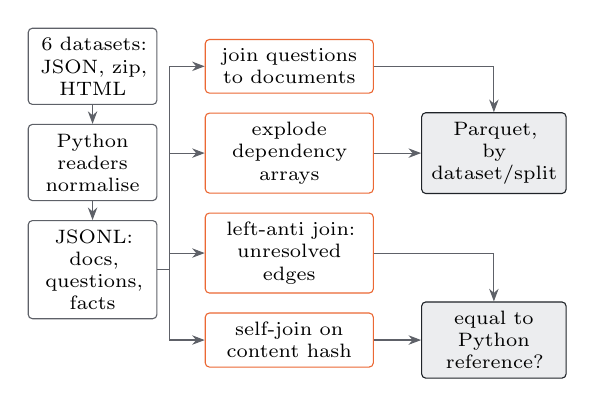
\begin{tikzpicture}[node distance=2.4mm and 3mm,font=\scriptsize,
  src/.style={draw=muted,rounded corners=1.5pt,fill=white,align=center,text width=14mm,minimum height=6mm},
  job/.style={draw=deporange,rounded corners=1.5pt,fill=white,align=center,text width=19mm,minimum height=6mm},
  sink/.style={draw=ink,rounded corners=1.5pt,fill=colhead!35,align=center,text width=16mm,minimum height=6mm}]
\node[src] (s1) {6 datasets:\\JSON, zip, HTML};
\node[src,below=of s1] (s2) {Python readers\\normalise};
\node[src,below=of s2] (s3) {JSONL: docs,\\questions, facts};
\node[job,right=6mm of s1] (j1) {join questions\\to documents};
\node[job,below=of j1] (j2) {explode\\dependency arrays};
\node[job,below=of j2] (j3) {left-anti join:\\unresolved edges};
\node[job,below=of j3] (j4) {self-join on\\content hash};
\node[sink,right=6mm of j2] (p) {Parquet,\\by dataset/split};
\node[sink,right=6mm of j4] (v) {equal to Python\\reference?};
\draw[flow] (s1)--(s2); \draw[flow] (s2)--(s3);
\foreach \j in {j1,j2,j3,j4}\draw[flow] (s3.east) -- ++(1.5mm,0) |- (\j.west);
\draw[flow] (j1.east) -| (p.north); \draw[flow] (j2)--(p);
\draw[flow] (j3.east) -| (v.north); \draw[flow] (j4)--(v);
\end{tikzpicture}
\caption{PySpark data layer. Spark SQL jobs in orange.}
\label{fig:spark}
\end{figure}

\textbf{Output.} The store holds 1,360,644 facts from 9,375 questions over 4,395
deduplicated documents, with 1,884,748 edges and 0 unresolved. The self-join found 491
identical document pairs across datasets, the measured reason we never pool. Parquet
uses 0.18~GB against 0.95~GB of JSON lines (5.1$\times$ smaller).

\textbf{Performance.} Table~\ref{tab:spark} times the same jobs at three data sizes and
1, 2, 4 and 8 cores on an eight-core laptop. On the full data Spark is fastest at four
cores, 37.0~s (36,700 facts/s), and slowest at eight, 65.6~s. Single-process Python
takes 15.8~s (86,000 facts/s). With 1.4 million rows and a 1.7~GB peak, the data fits
in memory, so JVM start-up, shuffles and collecting results to the driver for the
equality check are the likely overheads; we did not profile them. Parsing raw files into
facts takes 120~s in Python and is the real bottleneck. At this scale Spark contributes
a verified, partitioned columnar store, not speed, and we make no cluster scalability
claim.

\textbf{Batch evaluation.} The coverage audit runs 139,020 packings (9,268 questions
$\times$ 5 budgets $\times$ 3 methods) over eight worker processes in 679~s. A SQLite
ledger stores every model response under a frozen run contract (question IDs, seed,
input and code hashes), so runs resume after free-tier quota stops and re-scoring needs
no new calls.
\begin{table}[t]
\centering\footnotesize\setlength{\tabcolsep}{3pt}
\caption{Wall time (s): single-process Python and Spark on 1--8 cores. Size is records
per source dataset. All runs equal the Python reference.}
\label{tab:spark}
\begin{tabular}{lrrrrrrr}
Size & Facts & Python & 1 & 2 & 4 & 8 & Peak GB\\\hline\noalign{\vskip 2pt}
100 & 74,655 & 1.1 & 27.8 & 28.4 & 23.5 & 23.2 & 0.9\\
1000 & 507,594 & 6.0 & 23.4 & 21.2 & 20.2 & 33.4 & 1.4\\
full & 1,360,644 & 15.8 & 54.5 & 38.4 & 37.0 & 65.6 & 1.7\\
\end{tabular}

\end{table}

\section{Experimental setup}
\textbf{Budgets.} At 4,000 tokens four datasets were never truncated in a 40-question
sample, so the methods could not differ. We set each budget from document sizes, without
labels: 800 for FinQA and ConvFinQA and 400 for TAT-QA and TAT-HQA (the largest tested
values truncating about 70\% of sampled documents), and 1,500 for HybridQA and
MultiHiertt, which stay 93\% truncated even at 4,000.

\textbf{Measurements.} (1) The \emph{coverage audit} checks, with no model, whether every
gold operand or answer phrase survives packing; for the running example the gold
program is \texttt{divide(637, const\_5)}, so only 637 must survive. (2) \emph{Block A}
answers 50 questions per dataset with each of O, D and L (45 turns in 15 ConvFinQA
conversations). (3) \emph{Block B} compares the executor with direct answering on D
evidence, 40 questions per dataset.

\textbf{Model.} Table~\ref{tab:model} lists the configuration. Both models are used as
served, with no training or fine-tuning; each question is one API call, and the two
blocks are never compared with each other.

\textbf{Scoring.} Official execution accuracy for FinQA and ConvFinQA and official F1
elsewhere. Block B uses a 1\%-tolerance numeric measure for FinQA and ConvFinQA, since
direct answers have no program. Abstained and rejected answers score zero. Intervals
are paired bootstrap resamples of whole documents (2,000 resamples, seed 2626),
uncorrected across the six comparisons per block.
\begin{table}[t]
\centering\footnotesize\setlength{\tabcolsep}{3pt}
\caption{Model and inference configuration (from the frozen run contracts).}
\label{tab:model}
\begin{tabular}{lll}
\toprule
& Block A (packing) & Block B (executor)\\\midrule
Model & Gemini 3.5 Flash-Lite & Gemini 3.1 Flash-Lite\\
Served version & 3.5-flash-lite-07-2026 & 3.1-flash-lite-05-2026\\
Training & none (as served) & none (as served)\\
Output & schema-bound JSON & schema-bound JSON\\
Max output tokens & 2,048 & 2,048\\
Thinking level & low & low\\
Temperature & provider default & provider default\\
Responses & 885 & 472\\
Median tokens in / out & 1,403 / 129 & 1,214 / 109\\
Sample (seed 2626) & 50 per dataset & 40 per dataset\\
\bottomrule
\end{tabular}
\end{table}

\section{Results}
\subsection{Evidence coverage}
At the chosen budgets D keeps more gold evidence than O on all six datasets
(Table~\ref{tab:coverage}, Fig.~\ref{fig:coverage}). Questions kept by only one method
favour D 146 to 7 on HybridQA and 42 to 3 on MultiHiertt; FinQA (9 to 1) is weaker and
ConvFinQA (6 to 1) is not significant. The gap is largest where documents exceed the
budget most, and smallest on FinQA and ConvFinQA, where labels add only 7--8\% to a
document. It shrinks as the budget grows and is zero at 4,000 tokens on the four
smaller datasets. At 200 tokens the fixed cost of structure loses: $-1.8$ points on
ConvFinQA (36 against 63 discordant) and $-0.8$ on MultiHiertt (50 against 58). L is
below O at every budget, so extra neighbouring text does not substitute for labels.
\begin{table}[t]
\centering\footnotesize\setlength{\tabcolsep}{2pt}
\caption{Questions with all gold evidence retained (\%). D+/O+: kept only by D or only
by O; $p$: two-sided sign test.}
\label{tab:coverage}
\begin{tabular}{lrrrrrrr}
Dataset & $n$ & Cap & O & D & L & D+/O+ & $p$\\\hline\noalign{\vskip 2pt}
FinQA & 845 & 800 & 96.3 & 97.3 & 92.2 & 9/1 & 0.021\\
ConvFinQA & 1486 & 800 & 97.1 & 97.4 & 92.7 & 6/1 & 0.125\\
TAT-QA & 1636 & 400 & 90.1 & 91.7 & 82.6 & 41/15 & <.001\\
HybridQA & 3466 & 1500 & 72.0 & 76.0 & 67.7 & 146/7 & <.001\\
TAT-HQA & 792 & 400 & 84.2 & 86.9 & 75.4 & 33/12 & 0.002\\
MultiHiertt & 1043 & 1500 & 84.9 & 88.6 & 75.3 & 42/3 & <.001\\
\end{tabular}

\end{table}
\begin{figure*}[t]
\centering
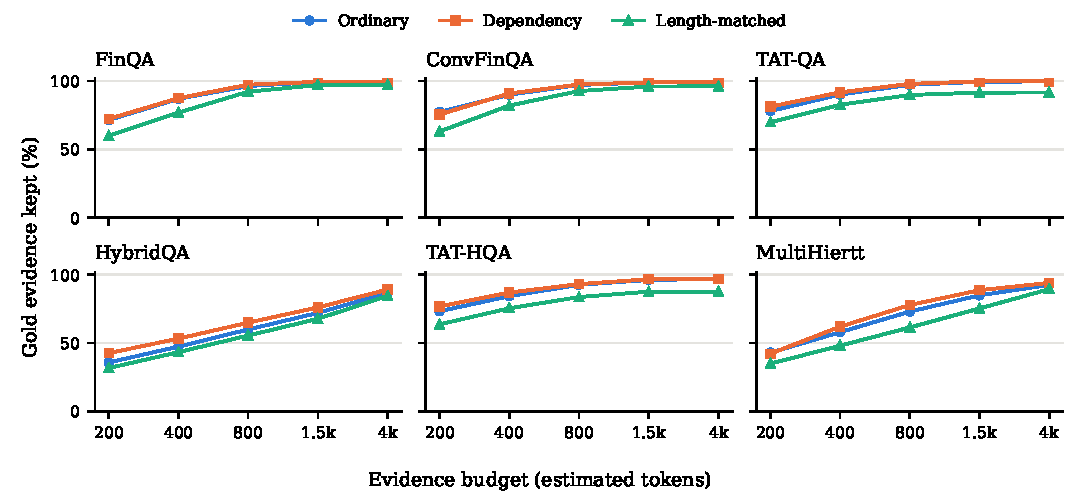
\includegraphics[width=.82\textwidth]{generated/coverage_wide.pdf}
\caption{Gold evidence retained against budget, full development splits.}
\label{fig:coverage}
\end{figure*}

\subsection{Effect on answers}
With Gemini 3.5 Flash-Lite, D scores at least as high as O on all six datasets, by 0 to
11.3 points (Table~\ref{tab:blocka}). Only TAT-QA's gain has an interval excluding
zero: +11.3 [+4.1, +19.9]. MultiHiertt (+9.8) and FinQA (+2.0) touch zero at the lower
bound. The pattern follows coverage: largest on hierarchical tables, absent on
ConvFinQA, whose documents nearly fit.

Fig.~\ref{fig:replay} replays one TAT-QA question with the saved model outputs: the
ratio of inventory reserves to accrued compensation in 2018, at a budget of 400. Both
methods pack the same two paragraphs (355 tokens). O fills the rest with three labelled
cells and stops at 398; the accrued-compensation cell, 358, needs 17 more tokens. The
model reports that the evidence lacks accrued compensation and abstains. D pays 33
tokens for the labels once and 3 per cell, fits 358, and the model's plan
\texttt{divide("948","358")} returns 2.65, the gold answer.
\begin{table}[t]
\centering\footnotesize\setlength{\tabcolsep}{2.2pt}
\caption{Block A answer scores (\%), Gemini 3.5 Flash-Lite. Execution accuracy for
FinQA and ConvFinQA, F1 otherwise.}
\label{tab:blocka}
\begin{tabular}{lrrrrrl}
Dataset & $n$ & O & D & L & D$-$O & 95\% CI\\\hline\noalign{\vskip 2pt}
FinQA & 50 & 62.0 & 64.0 & 66.0 & +2.0 & [+0.0, +6.2]\\
ConvFinQA & 45 & 73.3 & 73.3 & 68.9 & +0.0 & [$-$6.0, +6.4]\\
TAT-QA & 50 & 60.2 & 71.5 & 69.4 & +11.3 & [+4.1, +19.9]\\
HybridQA & 50 & 54.9 & 60.1 & 49.8 & +5.3 & [$-$2.4, +13.0]\\
TAT-HQA & 50 & 56.7 & 60.7 & 52.7 & +4.0 & [$-$6.4, +14.5]\\
MultiHiertt & 50 & 47.0 & 56.8 & 41.0 & +9.8 & [+0.0, +20.0]\\
\end{tabular}

\end{table}
\begin{table}[t]
\centering\footnotesize\setlength{\tabcolsep}{2.2pt}
\caption{Block B (\%), Gemini 3.1 Flash-Lite: executor against direct answering on D
evidence. MultiHiertt is official F1; under one numeric rule the gap is +6.2.}
\label{tab:blockb}
\begin{tabular}{lrrrrl}
Dataset & $n$ & Executor & Direct & Diff. & 95\% CI\\\hline\noalign{\vskip 2pt}
FinQA & 40 & 62.5 & 67.5 & $-$5.0 & [$-$17.5, +7.0]\\
ConvFinQA & 36 & 75.0 & 75.0 & +0.0 & [$-$8.6, +7.3]\\
TAT-QA & 40 & 65.2 & 58.7 & +6.5 & [$-$7.6, +20.7]\\
HybridQA & 40 & 50.2 & 66.6 & $-$16.4 & [$-$30.6, $-$2.0]\\
TAT-HQA & 40 & 60.0 & 56.7 & +3.3 & [$-$12.0, +19.3]\\
MultiHiertt & 40 & 63.7 & 41.7 & +22.1 & [+2.5, +40.0]\\
\end{tabular}

\end{table}
\begin{figure}[t]
\centering
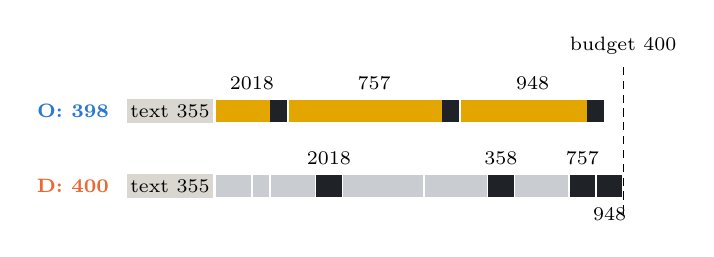
\begin{tikzpicture}[font=\scriptsize]
\node[anchor=east,text=ordblue,font=\scriptsize\bfseries,align=right] at (-0.1,0.15) {O: 398};
\fill[rule] (0,0.0) rectangle (1.1,0.30); \node at (0.55,0.15) {text 355};
\fill[rowlab] (1.130,0.0) rectangle ++(0.690,0.3);
\fill[ink] (1.820,0.0) rectangle ++(0.230,0.3);
\draw[white,line width=.5pt] (1.130,0.0) rectangle ++(0.920,0.3);
\node[above] at (1.590,0.30) {2018};
\fill[rowlab] (2.050,0.0) rectangle ++(1.955,0.3);
\fill[ink] (4.005,0.0) rectangle ++(0.230,0.3);
\draw[white,line width=.5pt] (2.050,0.0) rectangle ++(2.185,0.3);
\node[above] at (3.143,0.30) {757};
\fill[rowlab] (4.235,0.0) rectangle ++(1.610,0.3);
\fill[ink] (5.845,0.0) rectangle ++(0.230,0.3);
\draw[white,line width=.5pt] (4.235,0.0) rectangle ++(1.840,0.3);
\node[above] at (5.155,0.30) {948};
\node[anchor=east,text=deporange,font=\scriptsize\bfseries,align=right] at (-0.1,-0.80) {D: 400};
\fill[rule] (0,-0.95) rectangle (1.1,-0.65); \node at (0.55,-0.80) {text 355};
\fill[colhead] (1.130,-0.95) rectangle ++(0.460,0.3);
\draw[white,line width=.5pt] (1.130,-0.95) rectangle ++(0.460,0.3);
\fill[colhead] (1.590,-0.95) rectangle ++(0.230,0.3);
\draw[white,line width=.5pt] (1.590,-0.95) rectangle ++(0.230,0.3);
\fill[colhead] (1.820,-0.95) rectangle ++(0.575,0.3);
\draw[white,line width=.5pt] (1.820,-0.95) rectangle ++(0.575,0.3);
\fill[ink] (2.395,-0.95) rectangle ++(0.345,0.3);
\draw[white,line width=.5pt] (2.395,-0.95) rectangle ++(0.345,0.3);
\node[above] at (2.567,-0.65) {2018};
\fill[colhead] (2.740,-0.95) rectangle ++(1.035,0.3);
\draw[white,line width=.5pt] (2.740,-0.95) rectangle ++(1.035,0.3);
\fill[colhead] (3.775,-0.95) rectangle ++(0.805,0.3);
\draw[white,line width=.5pt] (3.775,-0.95) rectangle ++(0.805,0.3);
\fill[ink] (4.580,-0.95) rectangle ++(0.345,0.3);
\draw[white,line width=.5pt] (4.580,-0.95) rectangle ++(0.345,0.3);
\node[above] at (4.753,-0.65) {358};
\fill[colhead] (4.925,-0.95) rectangle ++(0.690,0.3);
\draw[white,line width=.5pt] (4.925,-0.95) rectangle ++(0.690,0.3);
\fill[ink] (5.615,-0.95) rectangle ++(0.345,0.3);
\draw[white,line width=.5pt] (5.615,-0.95) rectangle ++(0.345,0.3);
\node[above] at (5.788,-0.65) {757};
\fill[ink] (5.960,-0.95) rectangle ++(0.345,0.3);
\draw[white,line width=.5pt] (5.960,-0.95) rectangle ++(0.345,0.3);
\node[below] at (6.133,-0.95) {948};
\draw[densely dashed] (6.305,-1.15) -- (6.305,0.75) node[above] {budget 400};
\end{tikzpicture}

\caption{TAT-QA question at budget 400. Yellow: labels inline; dark: values; grey:
labels written once. O (398 tokens) has no room for 358; D (400) fits it.}
\label{fig:replay}
\end{figure}

\subsection{Executor against direct answering}
With Gemini 3.1 Flash-Lite, the executor gives no consistent gain
(Table~\ref{tab:blockb}). Direct answering leads on HybridQA by 16.4 points, with an
interval excluding zero; its answers are short text spans with no arithmetic. The
executor's 22.1-point lead on MultiHiertt is a scoring artefact: direct answers write
percentages ($-29.92$ for a gold $-0.2992$), which the official span path marks wrong.
Under one numeric rule for both sides the difference is +6.2 [$-6.2$, +20.0], so we
make no claim. The executor's value is that every answer traces to specific evidence.
Most remaining errors are wrong values, such as reversed percentage changes, or wrong
or over-long spans.

\section{Limitations}
Coverage measures presence, not correct use. Samples of 50 leave most per-dataset answer
gains within noise. Headers are inferred and can be wrong; budgets are estimated tokens;
BM25 misses paraphrases. Hosted models can change between runs. ConvFinQA and HybridQA
test labels are not public, so all results are on development splits.

\section{Conclusion}
Large tables must fit a model's fixed context window without losing what their numbers
mean. Writing each label once and linking every number to it keeps more of the evidence
a question needs at the same budget: on all six datasets at the chosen budgets, most
where documents exceed the budget, with a measured loss at 200 tokens. Answers from
Gemini 3.5 Flash-Lite follow, with a significant gain on TAT-QA. PySpark builds and
verifies the 1.36-million-fact graph the method runs on. Next steps are larger answer
samples, budget-aware closure that pays for a header only when several packed facts
share it, and better header inference for nested tables.

\bibliographystyle{IEEEtran}
\bibliography{references}
\end{document}
